\section{Δεδομένα}

\graphicspath{{Chapter4/Figs/Vector/}}

\begin{frame}
  \frametitle{Χρήση του Πακέτου 'tikz'}
  \framesubtitle{Προφανώς οι φωτογραφίες είναι από τα Τζουμέρκα!!}
  \label{fr4:hist_pics}
  
  \begin{tikzpicture}
    \node (img1) {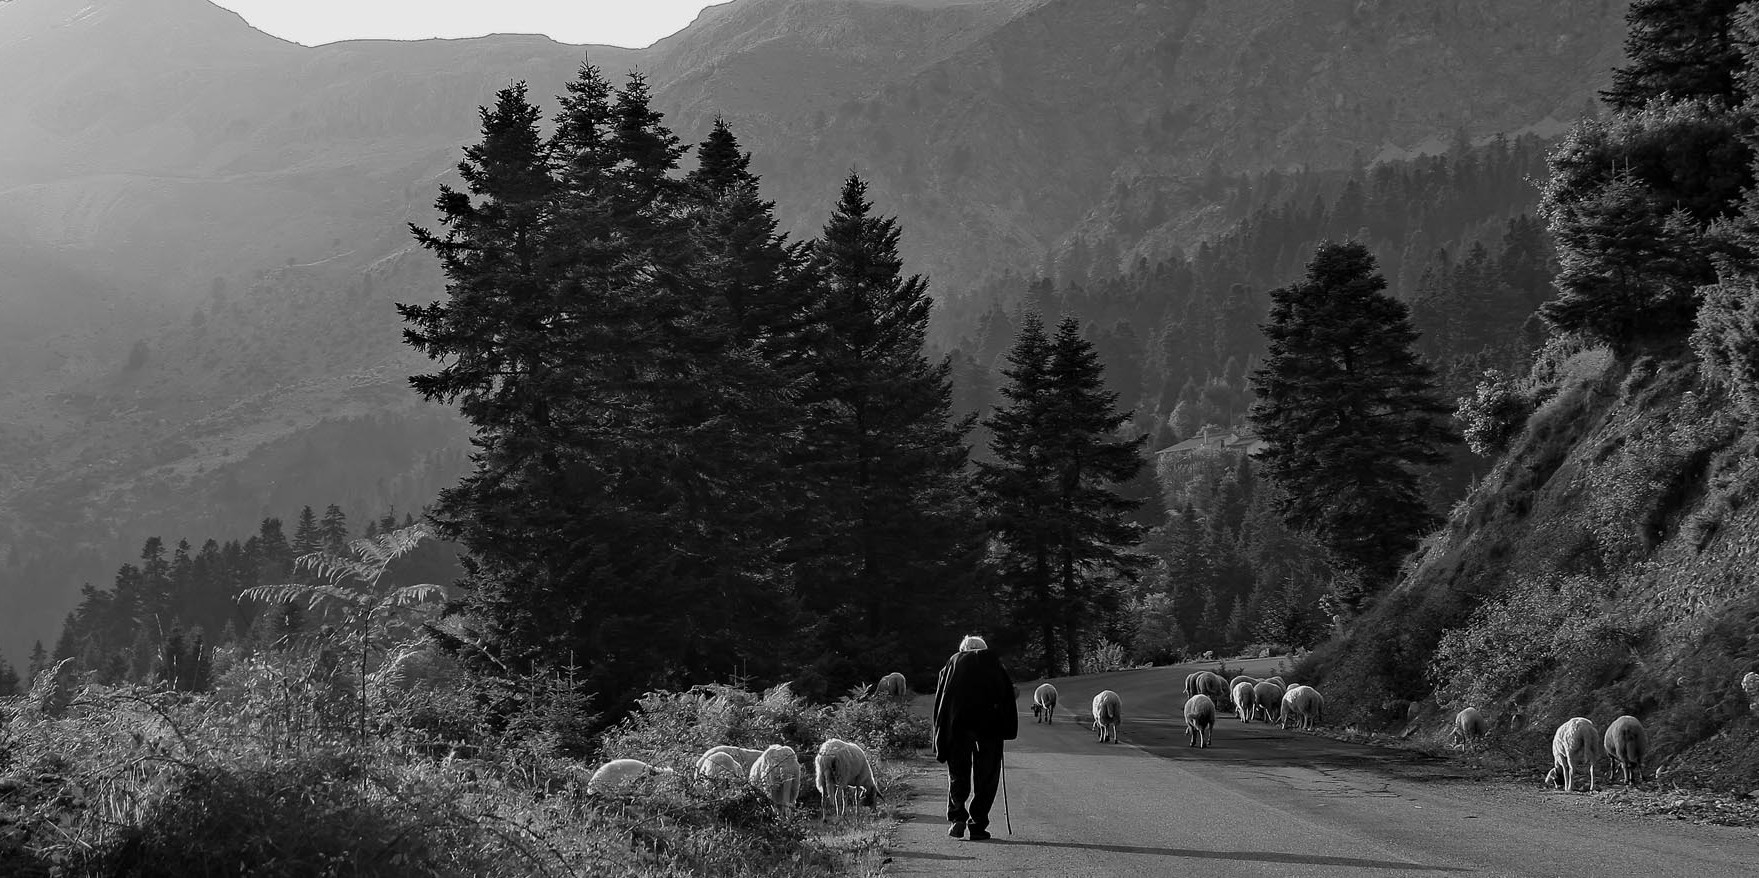
\includegraphics[height=3.6cm]{tsopanos.jpg}};
    \node (img2) at (img1.south west) [yshift=-1.2cm, xshift=.5cm]{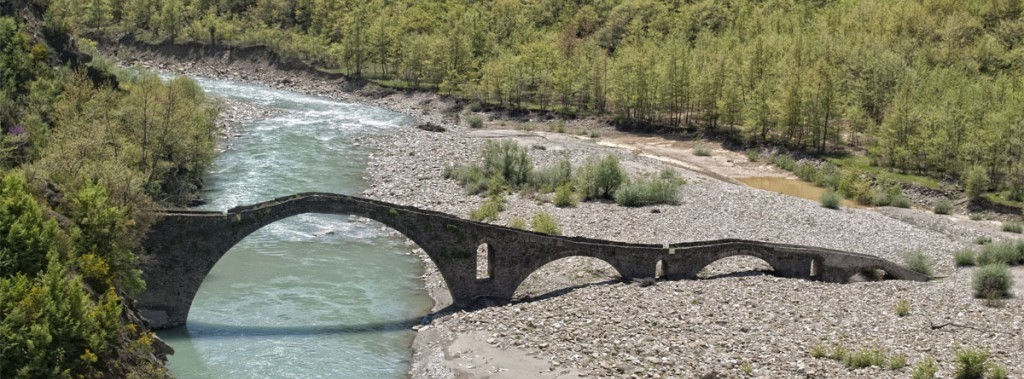
\includegraphics[height=3cm]{br-papastathi.jpg}};
    \node (img3) at (img2.north west) [yshift=1.7cm, xshift=1.5cm] {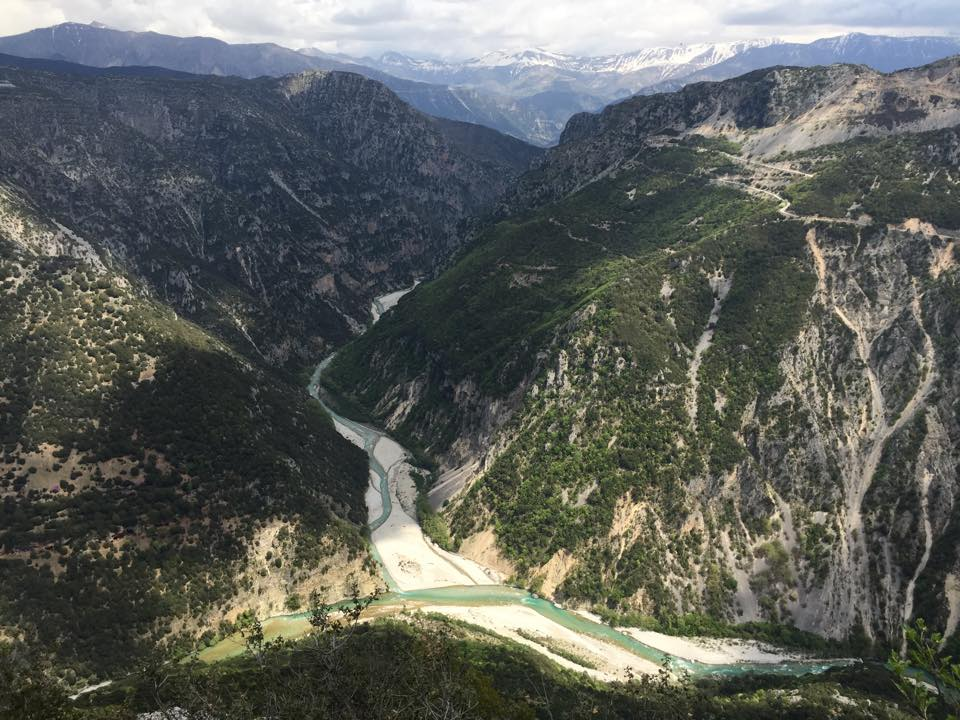
\includegraphics[height=3.2cm]{smiksi.jpg}};
    \node (img4) at (img2.east) [yshift=-.8cm,xshift=1.2cm] {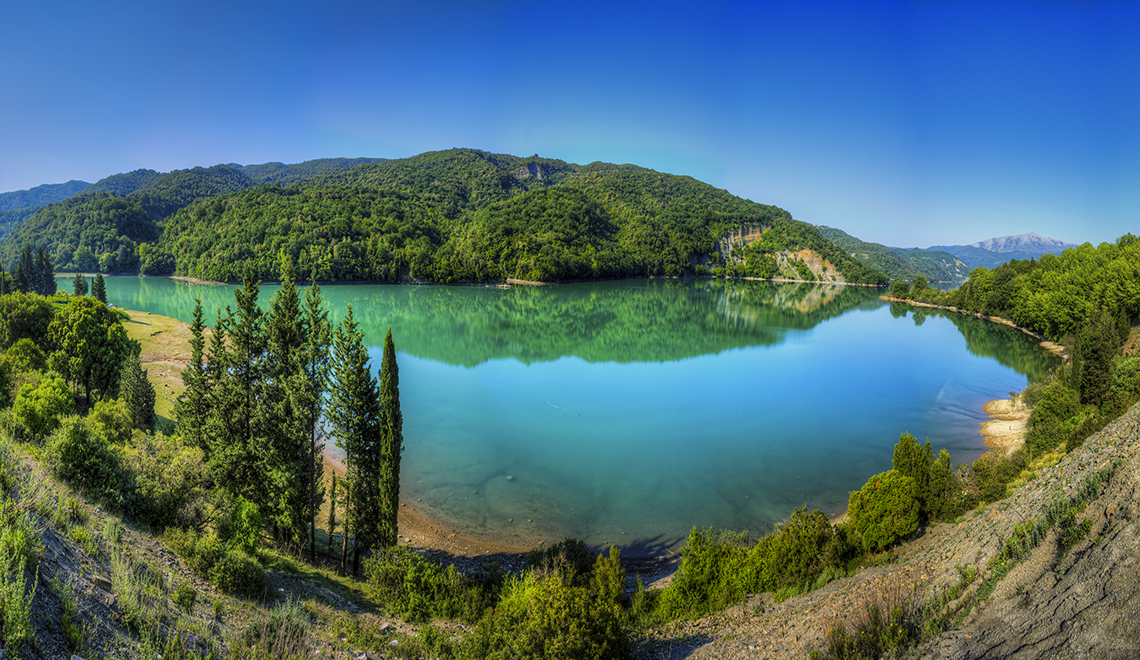
\includegraphics[height=1.8cm]{rouista.jpg}};
  \end{tikzpicture}
  

\end{frame}
\note{}
